\documentclass[12pt]{memoir}
\usepackage[spanish]{babel}
%\usepackage{geometry}
%\geometry{a4paper, margin=0.7in}
%\usepackage[final,1to1]{booklet}
% \usepackage{doclicense}
\usepackage[utf8]{inputenc}
\usepackage{baskervald}
\usepackage[T1]{fontenc}
\usepackage{graphicx}
\usepackage{wrapfig}
\usepackage{commath}

%opening
\title{Orientarse de noche}

\begin{document}

\maketitle
% 
\begin{abstract}
Orientarse no es sino obtener información que nos permita dirigir nuestros pasos (o nuestro coche, nuestro barco o nuestra nave espacial) en la dirección adecuada. Desde muy antiguo la humanidad se ha servido de los astros para encontrar esa información, pero el desarrollo de la tecnología (empezando por la invención de la brújula en el siglo IX d.C. en China, hasta los sistemas de posicionamiento global actuales) ha provocado el abandono paulatino de la orientación mediante signos naturales. No obstante, dada la relativa fragilidad de estos sistemas, es posible vernos envueltos en situaciones en las que sea preciso obtener la información suficiente para dirigir nuestro camino basándonos en la información que nos proporcione la propia Naturaleza y, de entre todas las señales que tenemos a nuestra disposición, las más fiables son las que recibimos a través de la observación del cielo.
\end{abstract}

\section{\textit{Cómo funciona} el firmamento}

Imaginemos que la Tierra se encuentra en un estadio de atletismo. El Sol está en el centro del estadio y nosotros estamos corriendo por la pista. Tardamos un año entero en dar una vuelta a la pista y cada día que pasa damos una vuelta sobre nosotros mismos. Las gradas del estadio son el fondo de estrellas del firmamento. 

% \vspace*{0.4in}

\begin{figure}[ht]
 \centering
 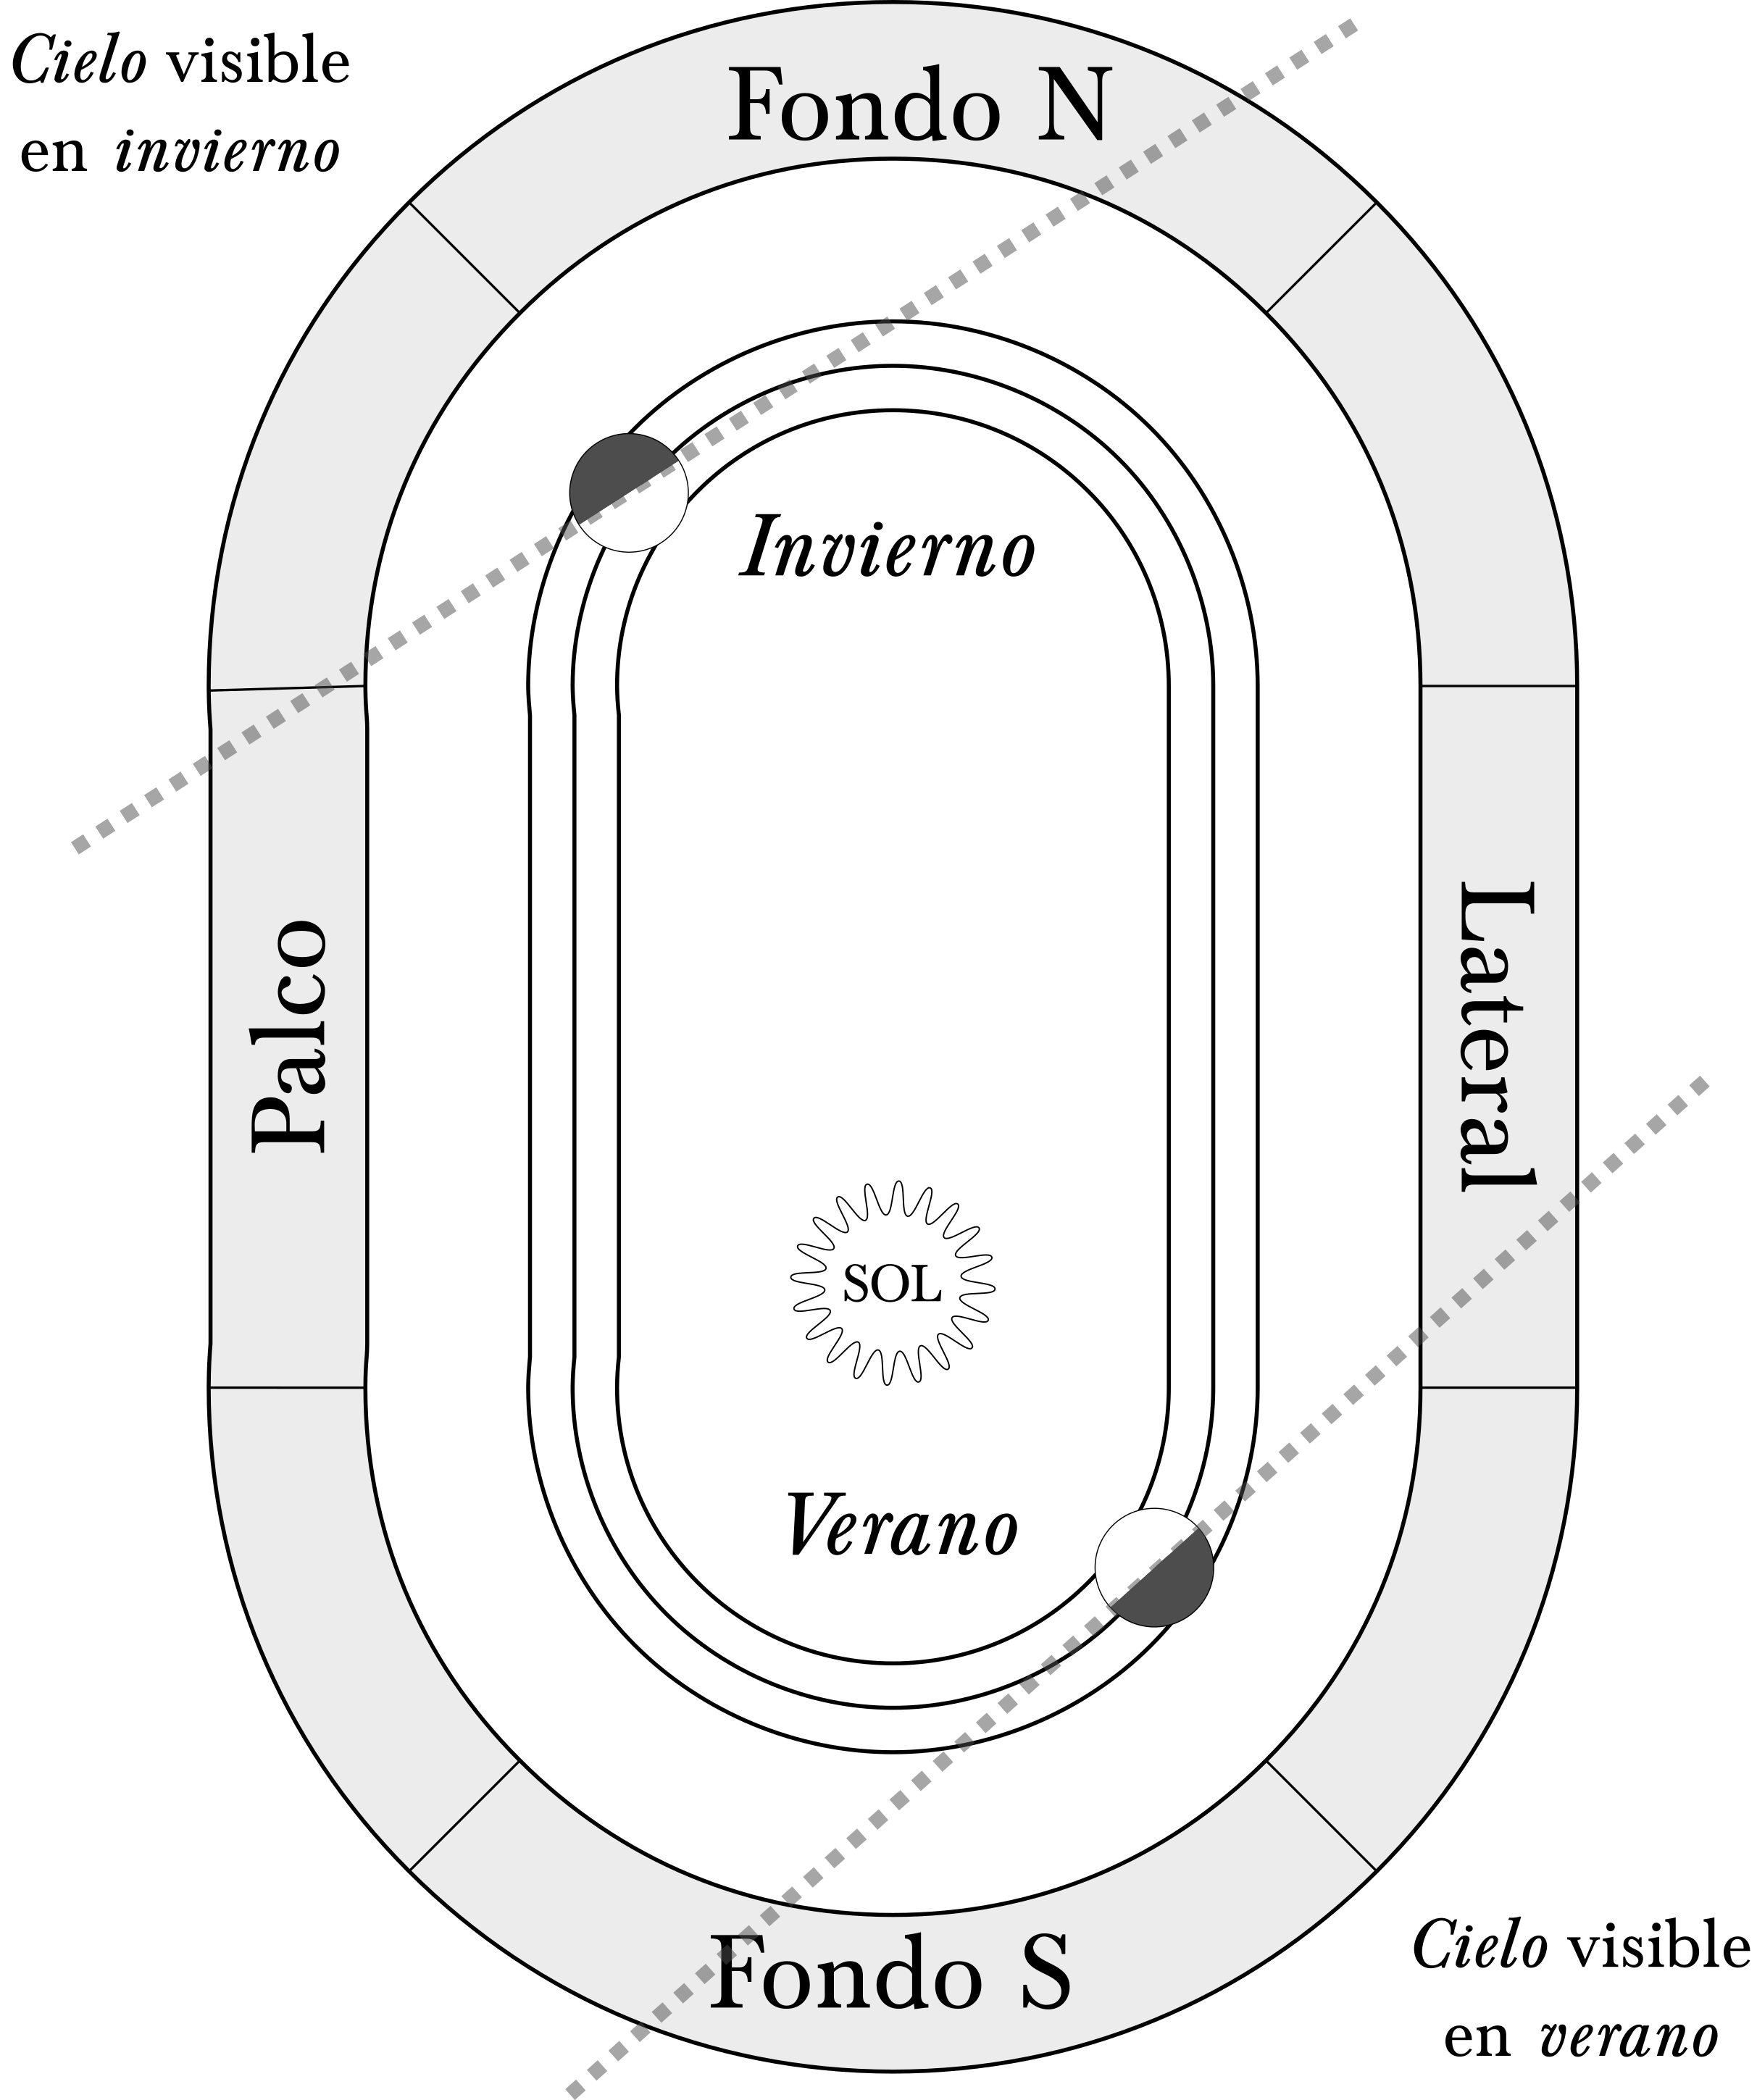
\includegraphics[width=200pt,keepaspectratio=true]{./esquema_firmamento.png}
 % esquema_firmamento.png: 0x0 pixel, 300dpi, 0.00x0.00 cm, bb=
 \caption{El movimiento de la tierra y el firmamento}
 \label{carrera_tierra}
\end{figure}

En esta peculiar carrera (\textit{la traslación terrestre}), cuando estamos mirando al centro del estadio miramos directamente al Sol (es de día). Su luz es tan fuerte que nos deslumbra y nos impide ver las gradas que quedan detrás de él, tal y como sucede en el mundo real; a medida que vamos girando y perdemos de vista el Sol aparece la noche. Es entonces cuando comenzamos a poder ver los graderíos (\textit{las constelaciones}) y todas las personas sentadas en ellos animando (\textit{los objetos celestes}) van apareciendo conforme giramos, pero dependiendo del lugar de la pista (la época del año) en la que nos encontremos estaremos mirando a diferentes graderíos y, por lo tanto veremos diferentes objetos celestes. Esta es la razón de que haya constelaciones que llamamos \textit{de invierno} y \textit{de verano}, ya que sólo son visibles de noche en cierta época del año.

El giro que efectuamos sobre nosotros mismos (\textit{la rotación terrestre}) provoca que los graderíos vayan apareciendo ante nuestros ojos siempre de la misma manera: aparecen por un punto cardinal (en el mundo real, por el Este) y desaparecen por el opuesto (el Oeste). Este giro se realiza en torno al eje de rotación terrestre, que atraviesa la Tierra y la esfera celeste por los polos. Como veremos más adelante, una de las claves para orientarse mediante las estrellas es localizar uno de los polos celestes, ya que inmediatamente se obtiene la dirección del polo terrestre correspondiente y de ahí el resto de los puntos cardinales.

\vspace*{0.4in}

\begin{figure}[ht]
 \centering
 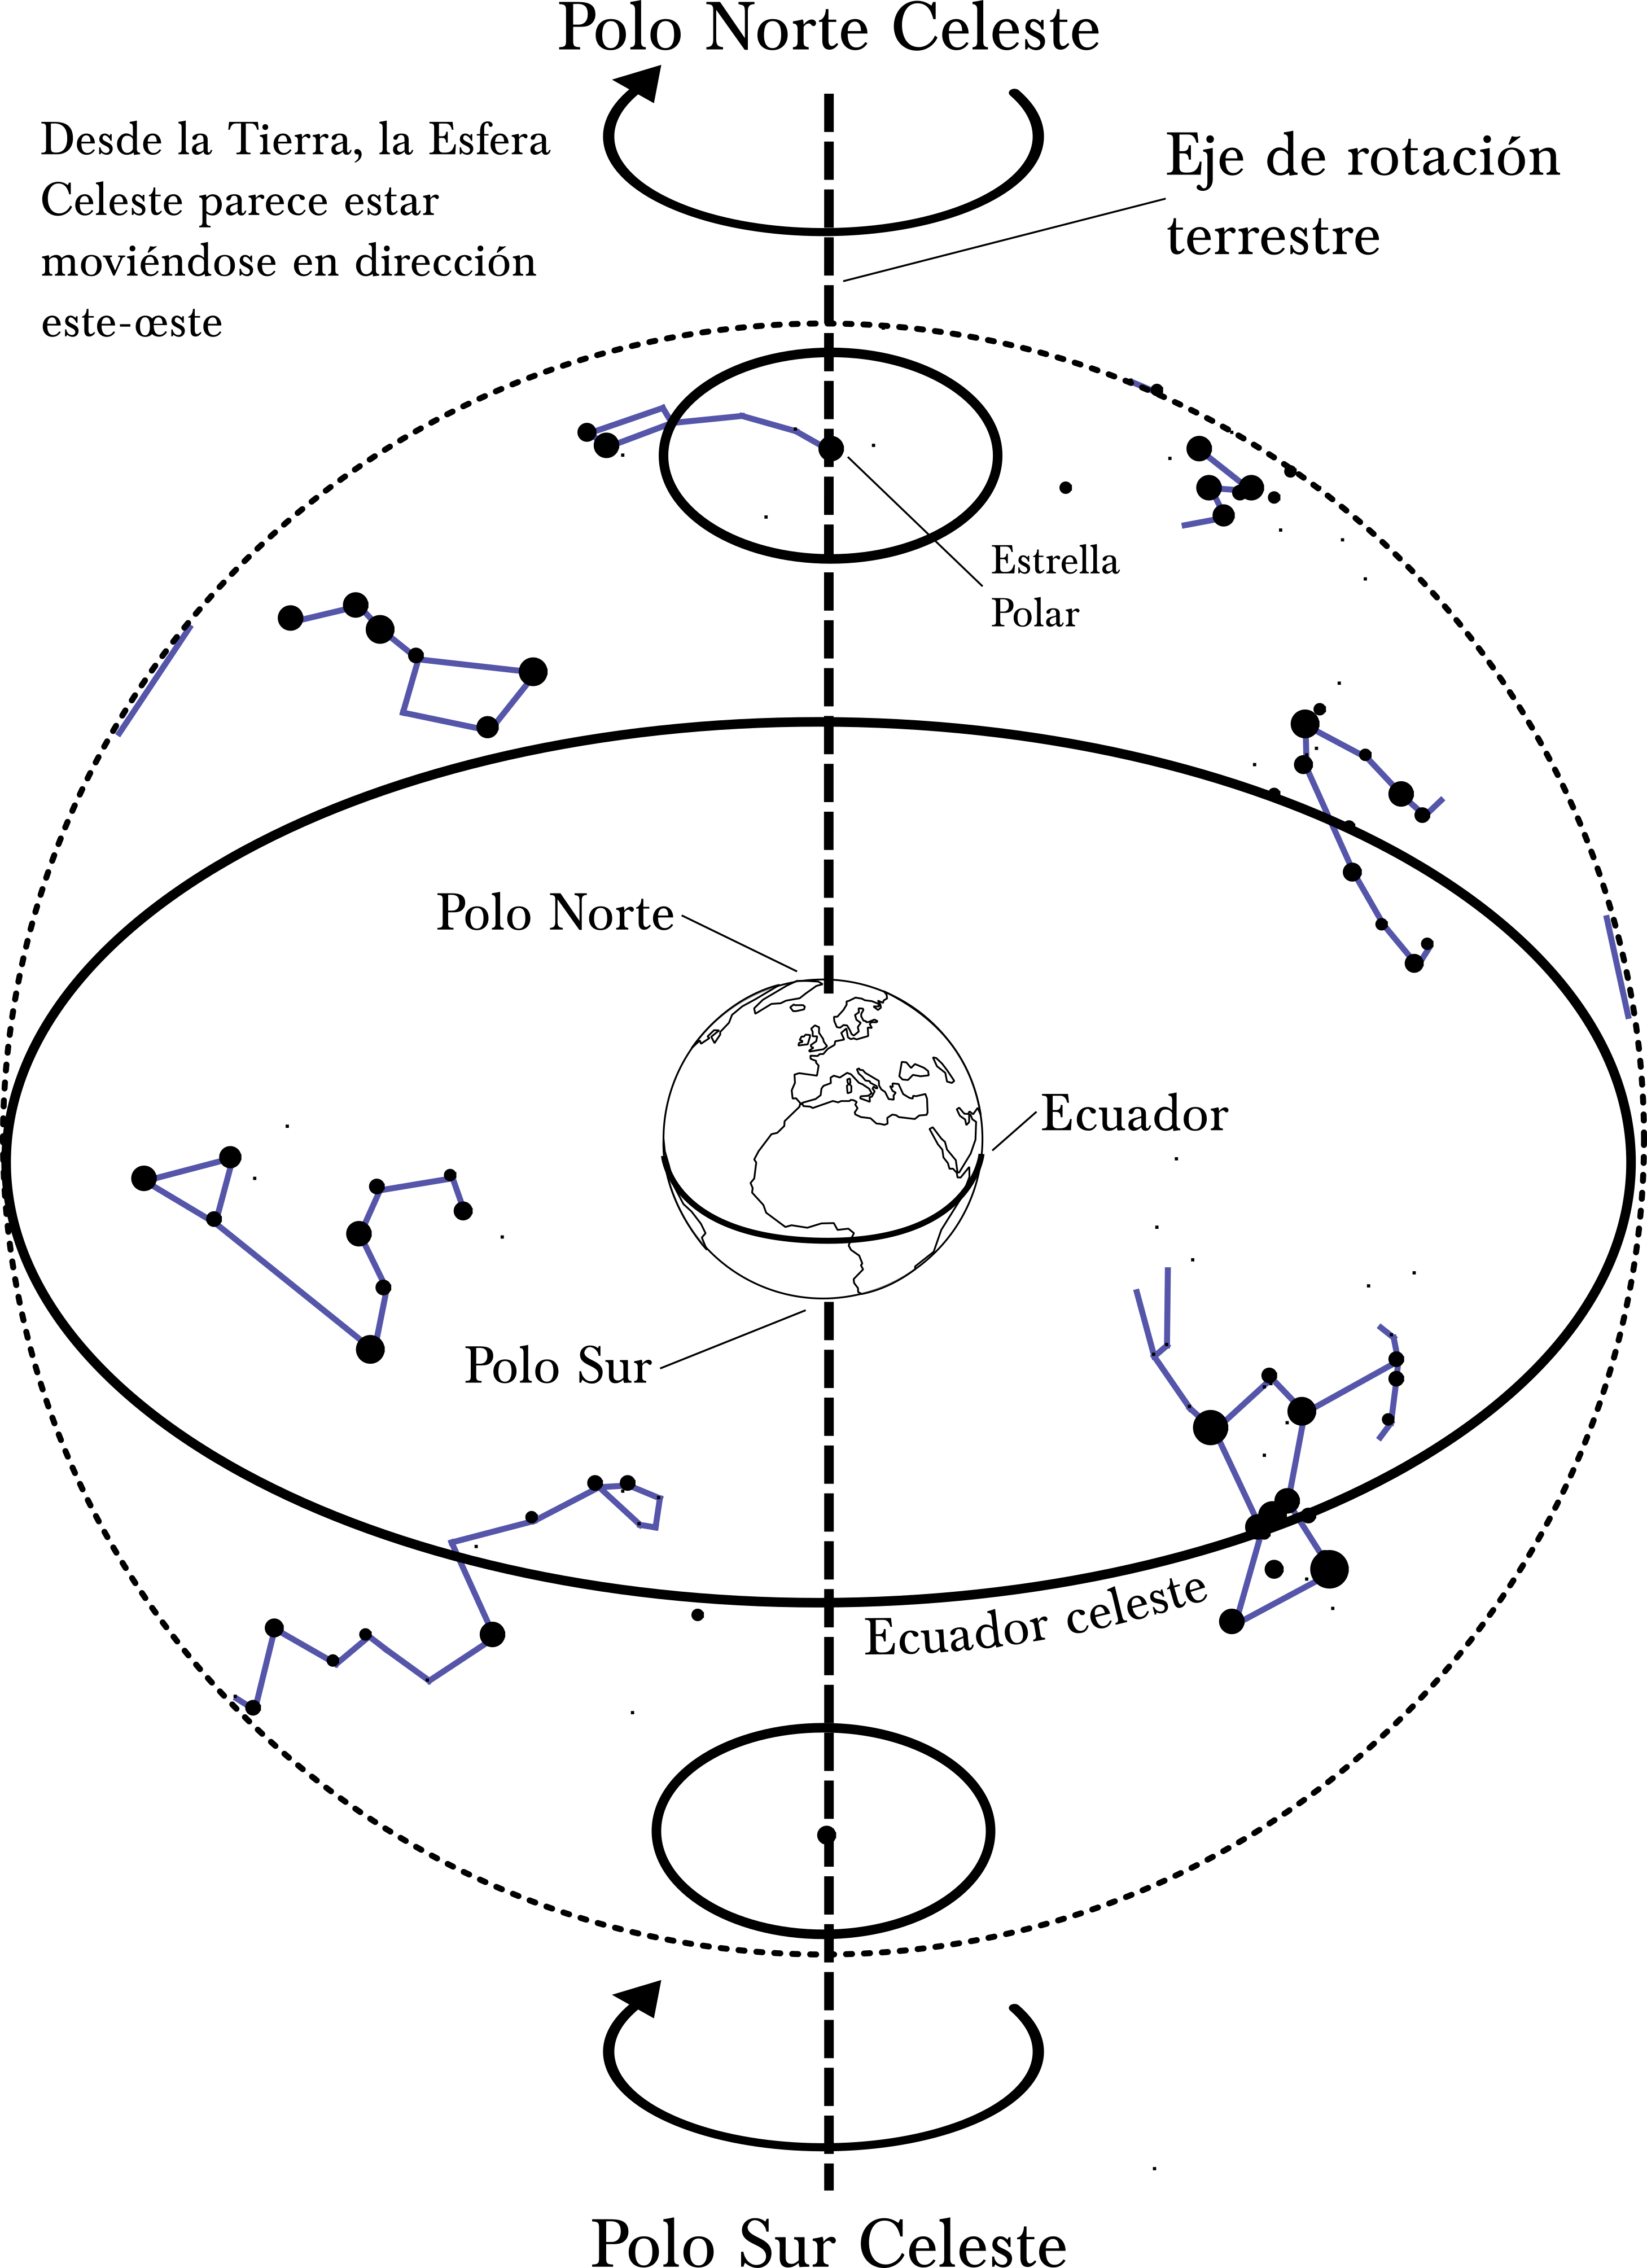
\includegraphics[width=250pt,keepaspectratio=true]{./esquema_cielo.png}
 % esquema_firmamento.png: 0x0 pixel, 300dpi, 0.00x0.00 cm, bb=
 \caption{La Tierra y la esfera celeste}
 \label{tierra_esfera}
\end{figure}


Por último, en el mundo real contamos con otro hecho que viene a complicar las cosas. Nuestro planeta tiene forma más o menos esférica, con lo cual no es lo mismo estar \textit{arriba}, en el hemisferio norte, que estar \textit{abajo}, en el hemisferio sur. Esta es la razón por la que no todos los objetos celestes y constelaciones son visibles en los dos hemisferios: ciertos objetos visibles desde posiciones del hemisferio sur no lo son desde el hemisferio norte, y viceversa. Esta es la razón por la que la localización de la estrella Polar no es un método de orientación útil en regiones australes.

\subsection{Situarnos en el cielo}

De igual manera que la posición de un punto sobre la tierra se identifica por sus coordenadas geográficas, la \textit{latitud} (en adelante la denotaremos como $\varphi$) y la \textit{longitud} (que denominaremos $\lambda$), en el caso de la esfera celeste, y empleando el sistema de coordenadas ecuatoriales, se emplea la \textit{declinación} (que abreviaremos como Dec. o $\delta$) y la \textit{ascensión recta} (abreviada como A.R. o $\alpha$), equivalentes a la latitud y la longitud, respectivamente.

\begin{figure}[ht]
 \centering
 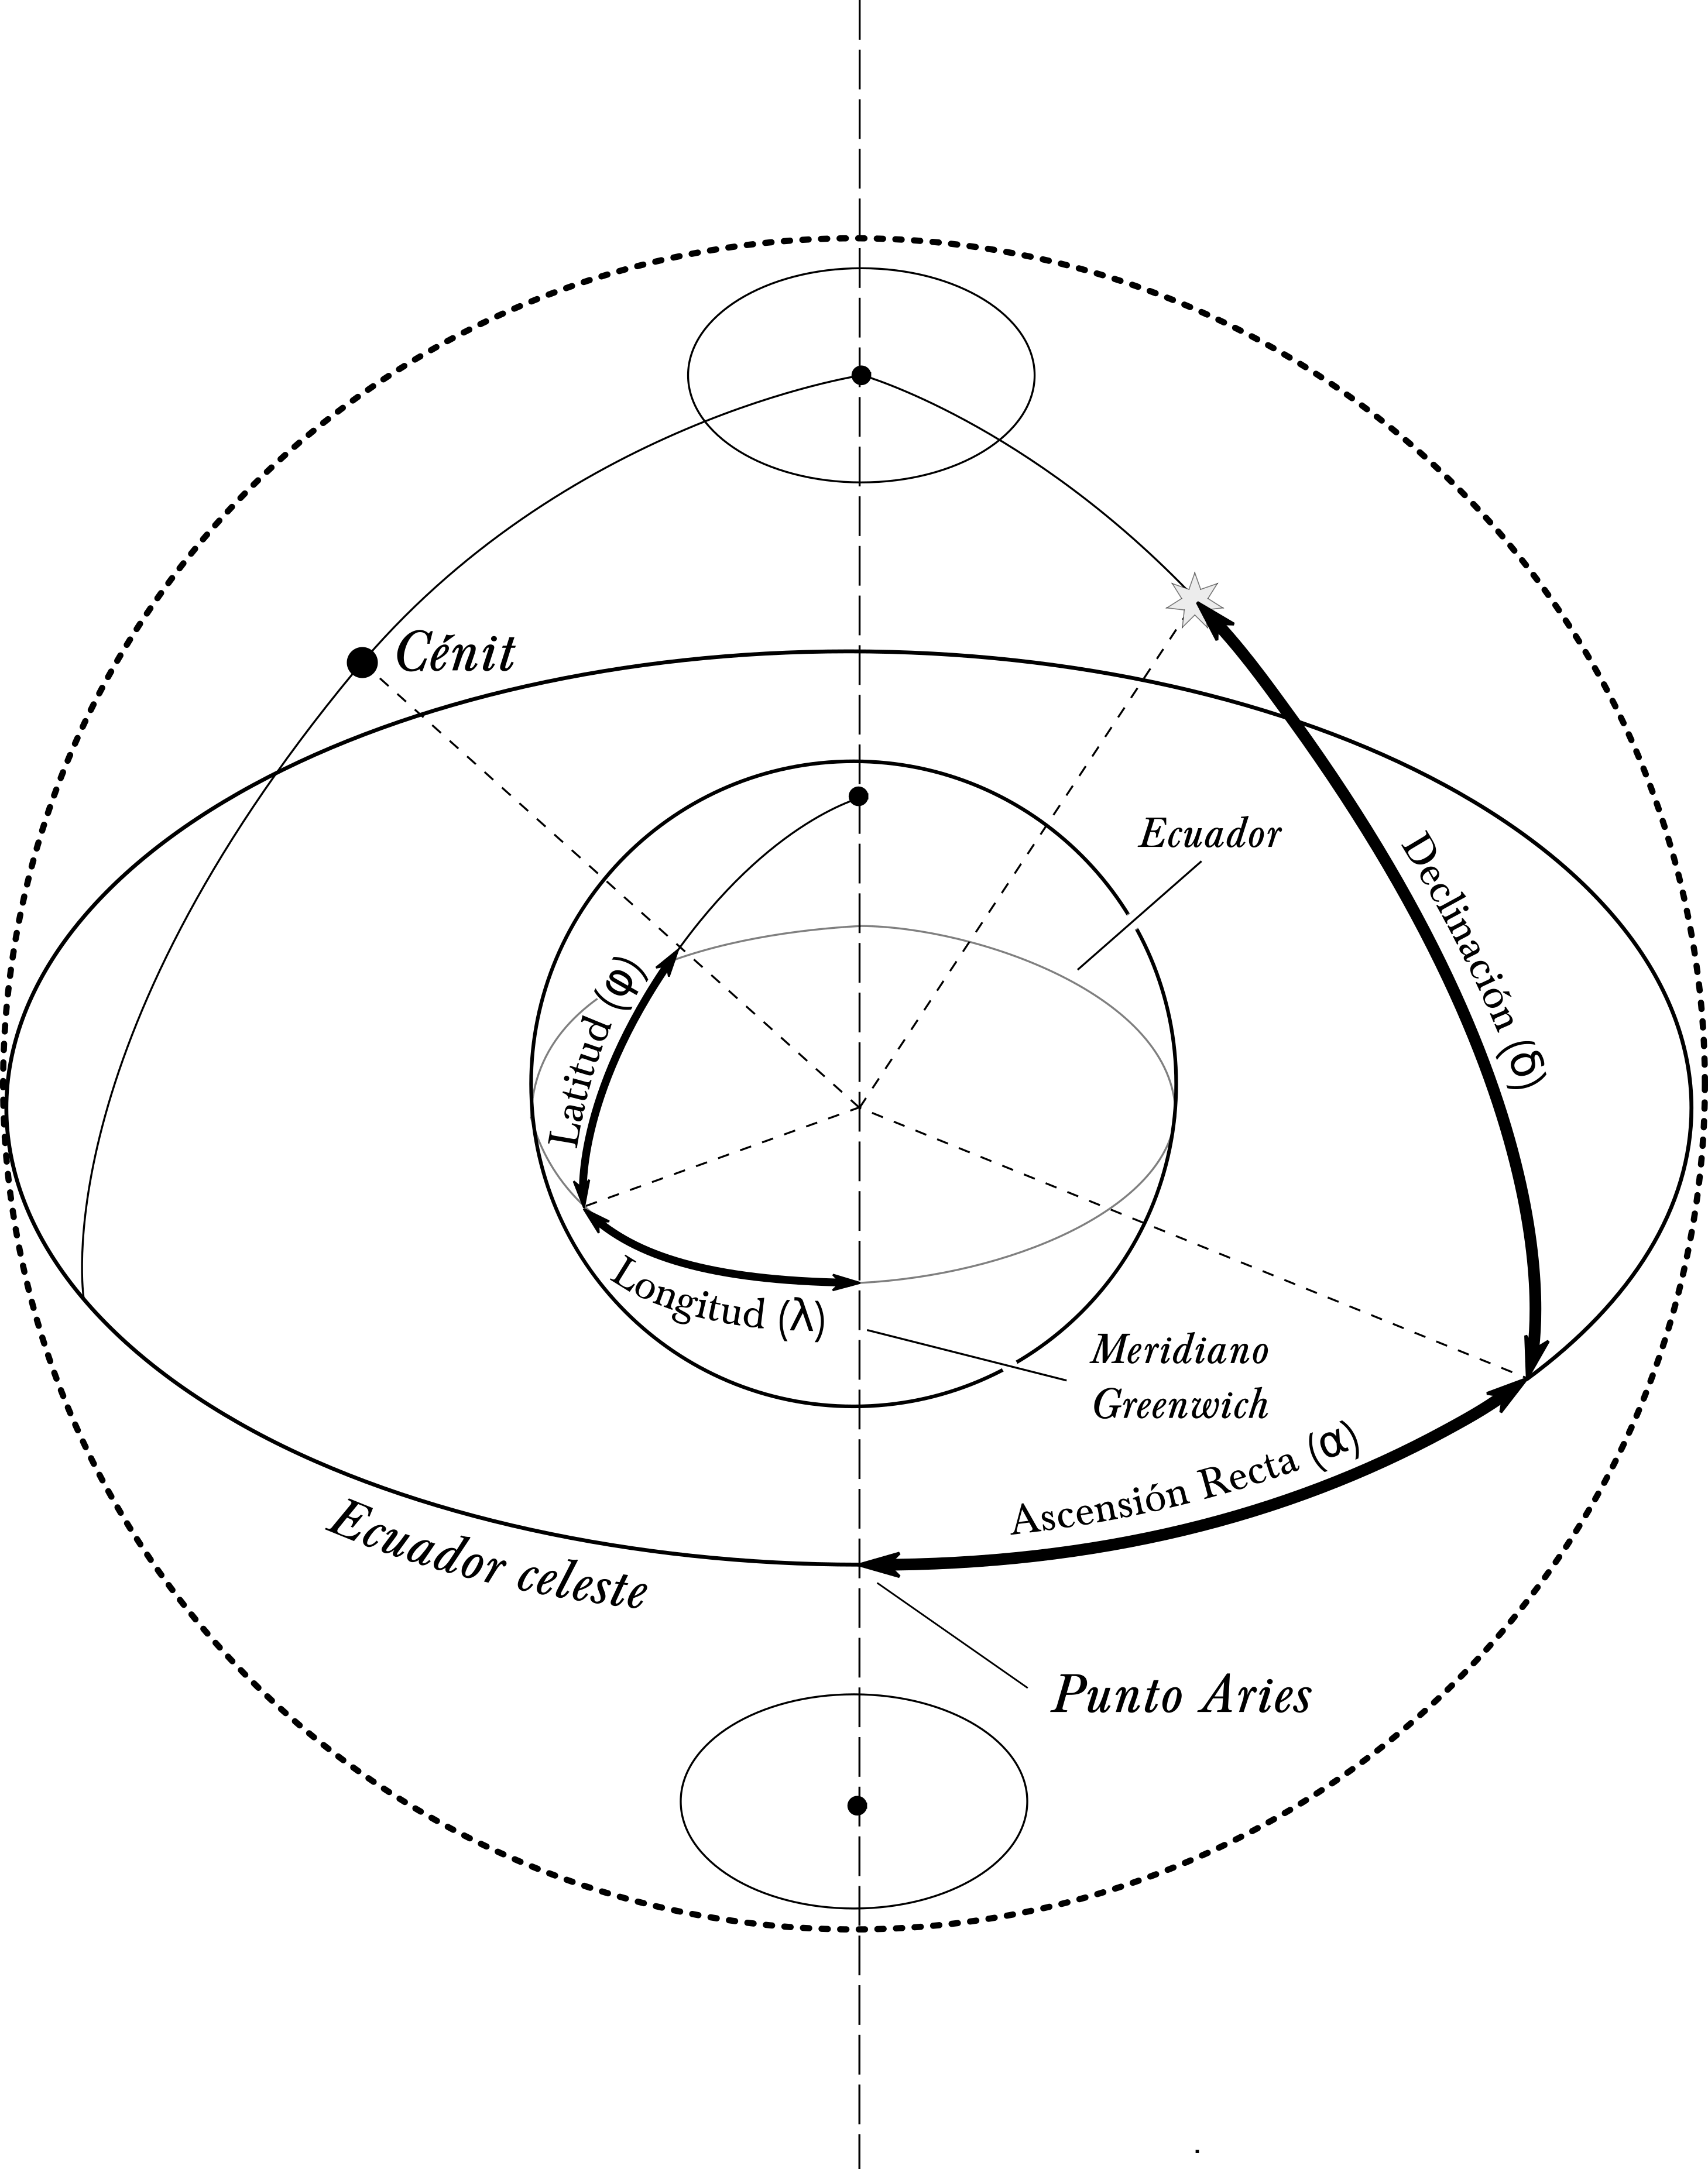
\includegraphics[width=250pt,keepaspectratio=true]{./coordenadas.png}
 % esquema_firmamento.png: 0x0 pixel, 300dpi, 0.00x0.00 cm, bb=
 \caption{Las coordenadas geográficas y celestes ecuatoriales}
 \label{coordenadas}
\end{figure}

Estos conceptos quedan ilustrados en la figura \ref{coordenadas}. Pero como todo sistema de coordenadas, es necesario definir el origen del sistema. En el caso de las coordenadas geográficas, el origen de la latitud es el ecuador terrestre; el de la longitud es el meridiano que pasa por el Observatorio de Greenwich, en Reino Unido. La latitud es positiva al norte del ecuador y negativa al sur; en cuanto a la longitud, es positiva hacia el este y negativa hacia el oeste.

En el caso de las coordenadas celestes ecuatoriales el origen de la declinación se encuentra en el ecuador celeste y el de la ascensión recta en el meridiano celeste que pasa por el denominado \textit{Punto Aries}, cuya definición se omitirá debido a su mayor complejidad. Mientras que la declinación se indica en grados, como en el caso de las coordenadas geográficas, la A.R. se indica en horas. Así, las coordenadas celestes de Mizar (una de las estrellas del carro de la Osa Mayor) son de Dec. = +54\textdegree 55' 31'' y su A.R. = 13 h 23 min 55.5 s. 

La declinación es positiva al norte del ecuador celeste y megativa al sur, de manera análoga a las coordenadas geográficas.

En la figura \ref{coordenadas} se identifica un punto del cielo conocido como \textit{cénit}, que corresponde al punto de la esfera celeste que está situado directamente encima del observador. Como se puede ver, la declinación del cénit coincide con la latitud del observador.

\subsection{El cielo según la latitud}


El movimiento aparente\footnote{Recordemos que el movimiento de los astros que observamos en el firmamento obedece a la rotación de la tierra y no al movimiento real de los mismos} de los objetos celestes es diferente según la latitud del observador. En general, la A.R. de los objetos visibles desde un punto dado de la Tierra es la comprendida 90\textdegree a cada lado del cénit. Como hemos dicho, la declinación del cénit corresponde a la latitud del observador, con lo cual:

\begin{itemize}
 \item Para el horizonte N, basta con restar a 90\textdegree el \textit{valor absoluto} de la latitud: 
 \[Dec. N = 90 - \abs{\varphi}\]
 \item Para el horizonte S, basta con sumar a -90\textdegree el \textit{valor absoluto} de la latitud:
 \[Dec. S = -90 + \abs{\varphi}\]
\end{itemize}


Si nos fijamos en la figura \ref{tierra_esfera}, el eje de rotación terrestre atraviesa la tierra y la esfera celeste por los polos. Si estuviéramos situados directamente sobre uno de los polos y pudiéramos visualizar ese eje sobre el terreno, lo veríamos salir del suelo y dirigirse a un punto concreto del cielo: el correspondiente polo celeste. Un observador situado en cualquiera de los dos polos terrestres ($\varphi$=90\textdegree  N o S), si mira hacia su cénit estará contemplando, por tanto, el polo celeste. 

Si nos encontrásemos en el hemisferio norte, tanto el horizonte sur como el norte se encontrarían en el ecuador celeste (ya que 90\textdegree - $\varphi$=0\textdegree) y, por tanto, las estrellas se moverían en círculos directamente encima del  observador y nunca se pondrían. Sólo son visibles los objetos celestes cuyas declinación estén comprendidas entre los 0º y los 90º, es decir, únicamente los situados en el hemisferio norte celeste, durante todas las noches del año\footnote{En el caso extremo de los polos, sólo hay una noche en el año, que dura 6 meses}. En el hemisferio sur ocurriría exatamente lo mismo, pero en este caso sólo veríamos los objetos australes.

Por el contrario, para un observador situado en el Ecuador ($\varphi$=0\textdegree), en los horizontes N y S se encuentran los respectivos polos celestes (ya que 90\textdegree - 0\textdegree = 90\textdegree y -90\textdegree + 0\textdegree = -90\textdegree) y por tanto el eje de rotación de la tierra atraviesa los horizontes N y S y el ecuador celeste se encuentra en el cénit, por lo que todos los astros salen y se ponen todos los días describiendo arcos por encima del observador con dirección este-oeste. Todos los objetos visibles por la noche en esa época del año son visibles para el observador\footnote{Consúltese la figura \ref{carrera_tierra}}.

En latitudes intermedias el panorama se complica. El polo celeste se encuentra a una altura sobre el horizonte igual a la latitud geográfica del lugar, y los horizontes N y S se encuentran a (90-$\Phi$)\textdegree de latitud N y S respectivamente. Suponiendo un lugar del hemisferio norte, esto tiene tres consecuencias importantes:

\begin{itemize}
 \item Todo objeto celeste situado entre los horizontes N y S saldrá y se pondrá todos los días y su visibilidad nocturna dependerá de la época del año.
 \item Todo objeto celeste situado por debajo del horizonte S no saldrá ni se pondrá nunca.
 \item Todo objeto celeste situado por encima del horizonte N nunca se pondrá y será visible durante todas las noches del año.
\end{itemize}

A estos últimos objetos se les denomina \textit{circumpolares}, y son de capital importancia para la orientación mediante las estrellas ya que siempre son visibles sobre el horizonte y, por lo tanto, siempre están disponibles para orientarnos.

Por ejemplo, para el caso de Cádiz, cuya $\varphi$=36.5\textdegree, el polo celeste se encuentra al 36,5\textdegree sobre el horizonte, aproximadamente, por lo que los horizontes N y S se encuentran a  90\textdegree - 36.5\textdegree = 53.5\textdegree de latitud N o S. Todas los objetos situados por debajo de la latitud 53.5\textdegree S no serán visibles nunca. Los objetos entre los 53.5\textdegree de latitud S y los 53.5\textdegree de latitud N tendran su orto y ocaso diario, mientras que los comprendidos entre los 53.5\textdegree y 90\textdegree de latitud N serán circumpolares.

En el caso del hemisferio sur el fenómeno es idéntico, salvo que los objetos circumpolares los son con respecto al polo celeste sur y los objetos invisibles se encuentran en el hemisferio norte. 

\section{La orientación mediante el firmamento}

Como se dijo en la introducción orientarse es obtener la información suficiente que permita  dirigir nuestro camino en la dirección adecuada. Esto significa ser capaz de localizar sobre el terreno los puntos cardinales y usar esa información para leer correctamente un mapa o, mediante los conocimientos de la zona en la que nos encontramos,

No todos los métodos de orientación son igual de precisos: algunos de precisión relativamente alta no están siempre disponibles y/o son relativamente prácticos debido a que la obtención de resultados conlleva esperas prolongadas. Pero por diferentes razones puede ser necesario hacer uso de métodos menos fiables si las condiciones lo requieren. 

En general se debe tratar de emplear siempre el método más preciso en función de las circunstancias existentes. Así, por ejemplo, no tiene sentido intentar orientarse por la estrella Polar en latitudes muy próximas al ecuador o del hemisferio sur, o en un valle cuyas montañas la oculten. En estos casos, deberemos buscar un método alternativo escogiendo aquel que nos permita una mejor localización de los puntos cardinales.



\end{document}
